\section{The Large Hadron Collider}
The Large Hadron Collider (LHC)~\ref{cern-faq} is the largest and most powerful particle collider that has ever been built. Construction of the LHC involved a collaboration of more than 10,000 scientist from more than 100 countries and was completed in 2008, after a decade of work. The cost of the machine alone is about 5 billion USD (3 billion Euro).

The European Organization for Nuclear Research (CERN) built the LHC in a tunnel underneath the border of France and Switzerland, near the city of Geneva. The LHC occupies a large tunnel 27 km in circumference that was originally constrcted in the 1990s for the Large Electron Positron collider (LEP). Hadrons (either protons or ions) are accelerated and focused into two beams traveling in opposite directions around this tunnel. These beams are then made to collide with very high energy at one of the four collision points along the ring where their paths intersect. AEach of these points is home to one of the four main LHC experiments: A Large Ion Collider
Experiment (ALICE)~\cite{cern-jinst-alice}, ATLAS~\cite{cern-jinst-atlas}, the Compact Muon Solenoid (CMS)~\cite{cern-jinst-cms}, and the Large Hadron Collider beauty (LHCb) experiment~\cite{cern-jinst-lhcb}. ALICE is a detector that looks at collisions of lead ions to study the properties of quark-gluon plasma. ATLAS is a general-purpose detector that looks for a wide range of possible new types of physics, including the Higgs boson, supersymmetry (SUSY) and extra dimensions. CMS is an additional general-purpose detector, designed and run independently from ATLAS, but with the same goals in mind. LHCb is a detector specially designed to study the asymmetry between matter and anti-matter in the interactions of B-particles. Figure~\ref{fig:lhc-exp} shows a aerial view diagram with the locations of these four experiments along the LHC ring. The location of the LHC ring in relation to the city of Geneva and the French-Swiss border is also illustrated.

\begin{figure}[tp]
  \centering
  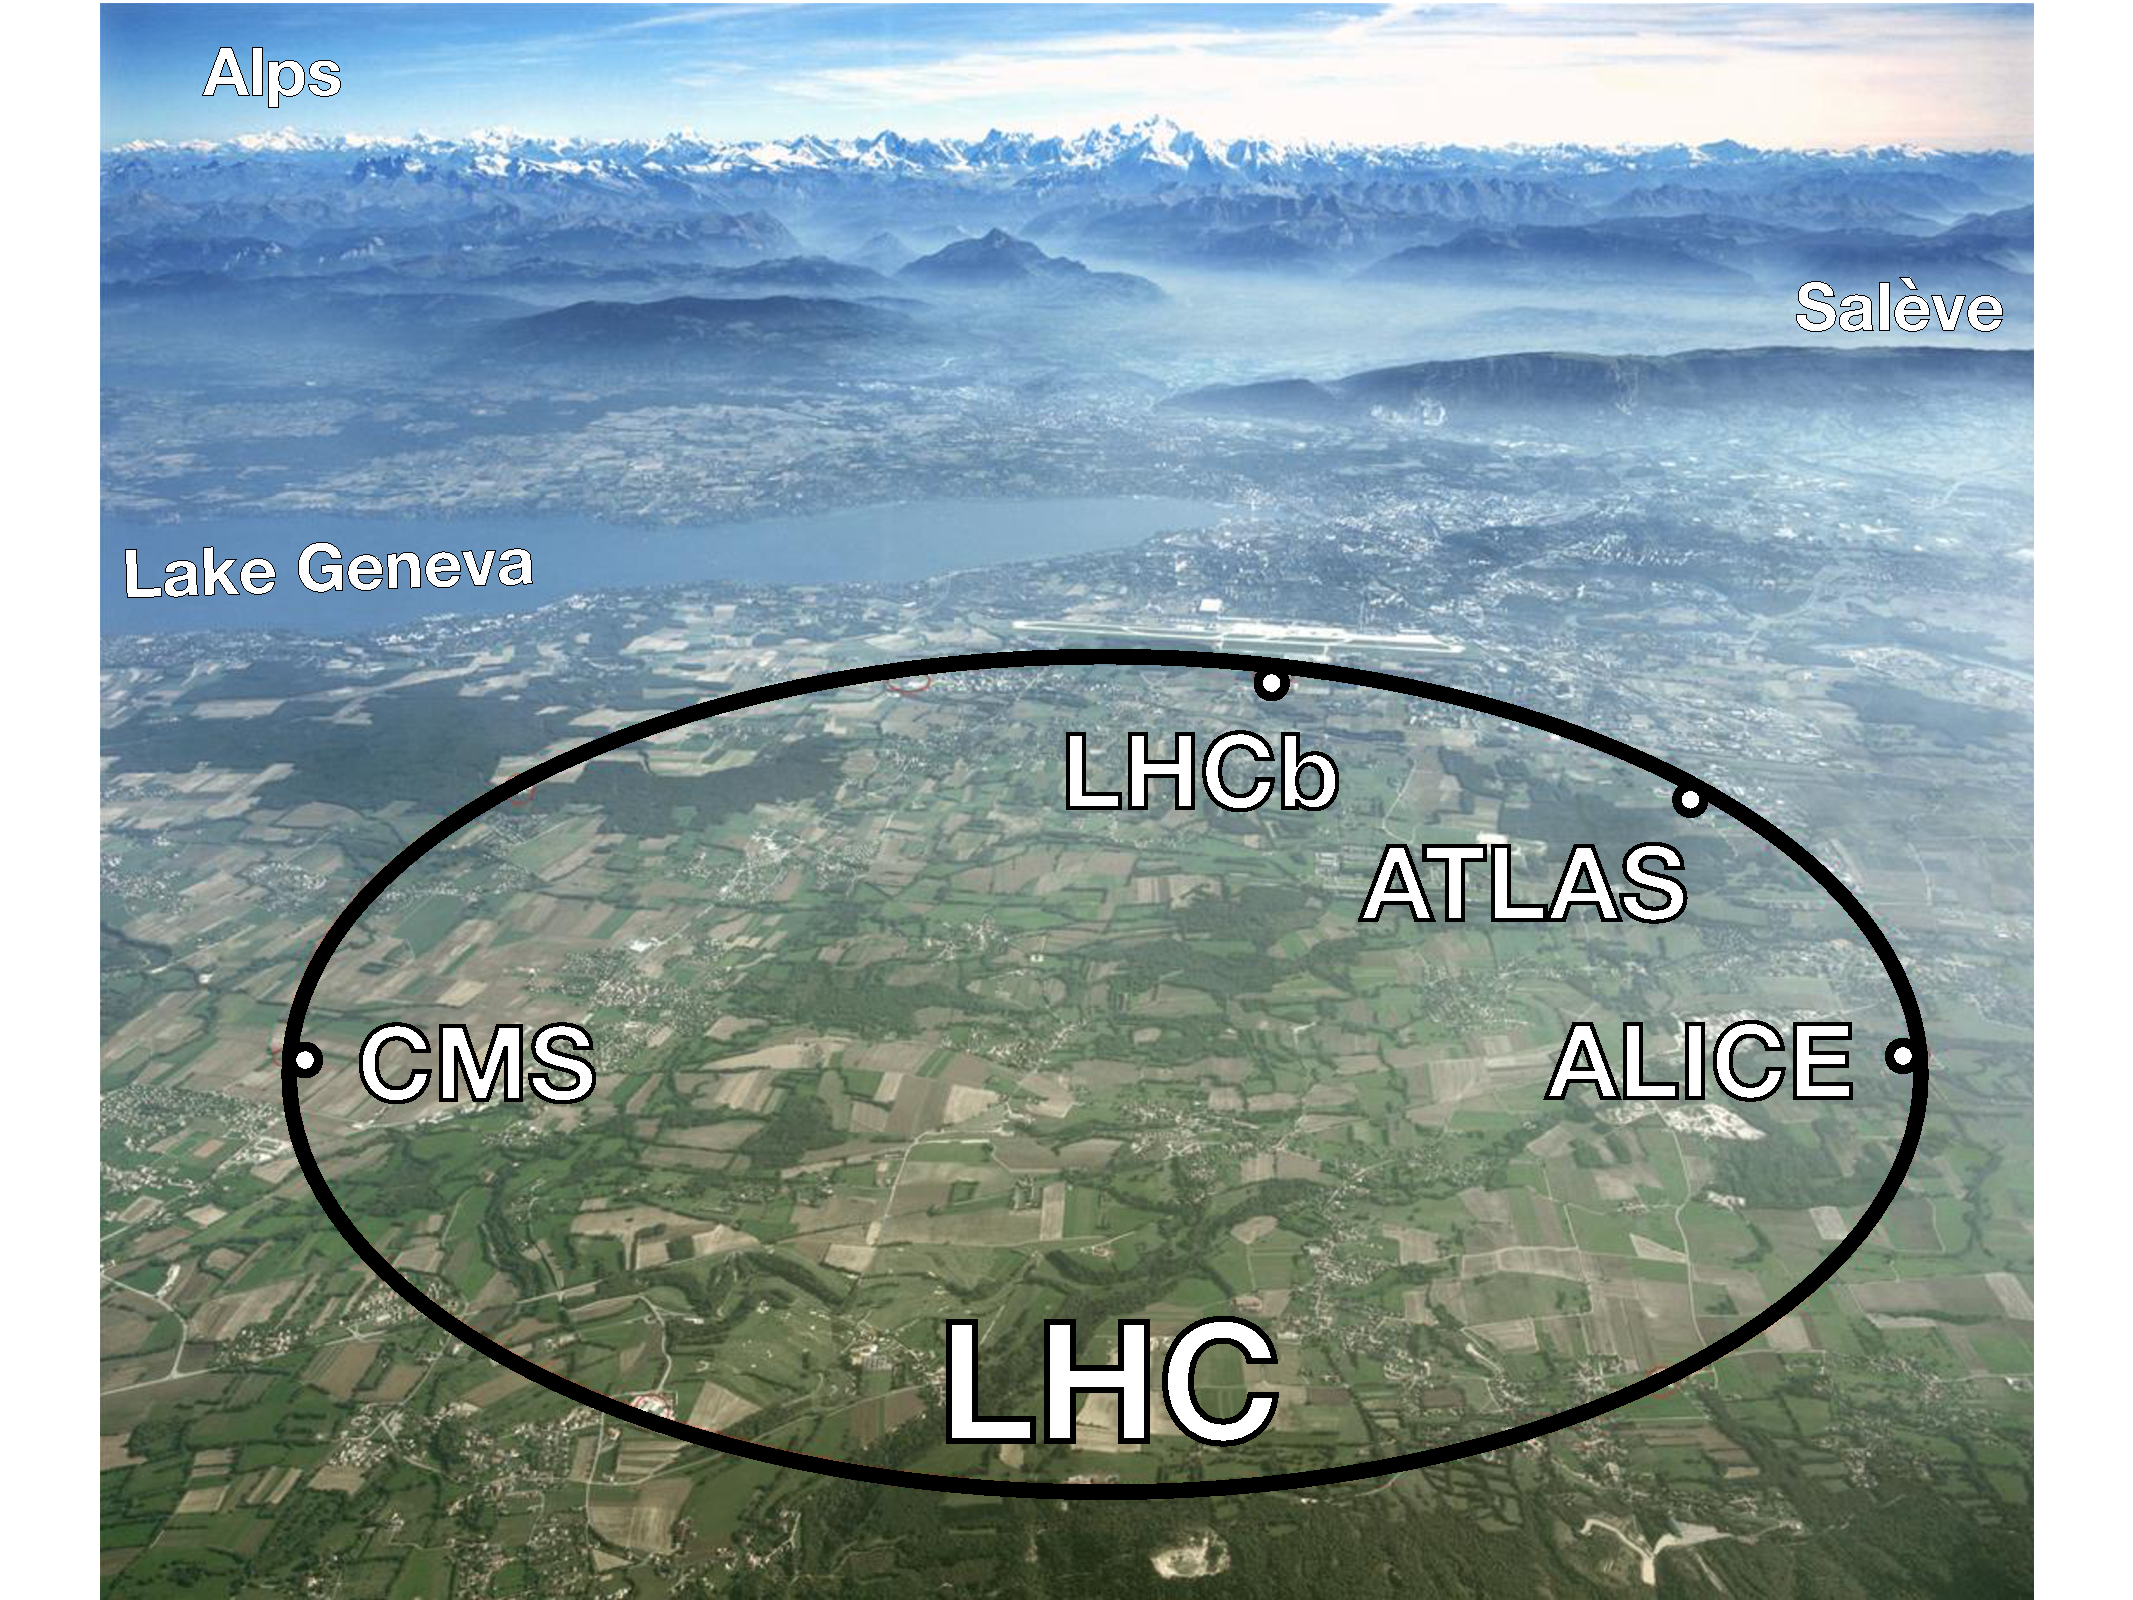
\includegraphics[width=0.90\textwidth]{fig/atlas/lhc-aerial.pdf}
  \caption{The location of the four main LHC experiments: ALICE, ATLAS, CMS and LHCb. The LHC tunnel is 27 km in circumference, situated underneath the border of France and Switzerland, near the city of Geneva, as shown.~\cite{atlas-surface}.}
  \label{fig:lhc-exp}
\end{figure}

The main goal of the LHC is to investigate unsolved questions in our current understanding of particle physics, such as the details of the Higgs mechanism, the existence of new particles from SUSY or extra dimensions and the source of dark matter and dark energy.
\subsection{Accelerator Complex}
A succession of machines known as the ``accelerator complex'' accelerate particles to increasingly higher energies~\cite{cern-jinst-lhc}, shown in Figure~\ref{fig:lhc-chain}. First, an electric field is used to strip protons from atoms in a simple bottle of hydrogen gas. Then, the first accelerator in the chain, Linac 2, accelerates protons to 50 \mev. Next, the beam is injected into the Proton Synchrotron Booster (PSB) and then the Proton Synchrotron (PS), which accelerate the protons to 1.4 \gev and 25 \gev respectively. After that, the Super Proton Synchrotron accelerates the protons to 450 \gev. The last step in the chain is the LHC; from the SPS, protons are transferred into the two beam pipes of the LHC and accelerated in opposite direction. Filling each of the rings of the LHC takes 4 minutes and 20 seconds, and it takes another 20 minutes to accelerate each beam to its final energy of 4 \tev. The same two beams will circle for many hours.

Inside the LHC, the beams travel in opposite directions around separate rings called ``beam pipes,'' which are tubes kept at ultrahigh vacuum. The beams are directed by a collection of very strong superconducting electromagnets, including 1232 dipole magnets and 392 quadrupole magnets. Superconduction requires the magnets to be cooled to -271.3 C. A distribution system of liquid helium keeps the magnets cool. The 15 meter long dipole magnets steer the beams around the ring, while the 5-7 meter long quadrupole magnets focus the beams before collision. The protons in the beams circulate in well-defined groups called \textit{bunches}. Each bunch consists of approximately $10^{11}$ particles, and each beam has 2808 bunches. This bunch structure maximizes the chances of collisions since multiple protons have the chance to collide each crossing. In 2012, bunch crossings occurred every 50 nanoseconds.




\begin{figure}[tp]
  \centering
  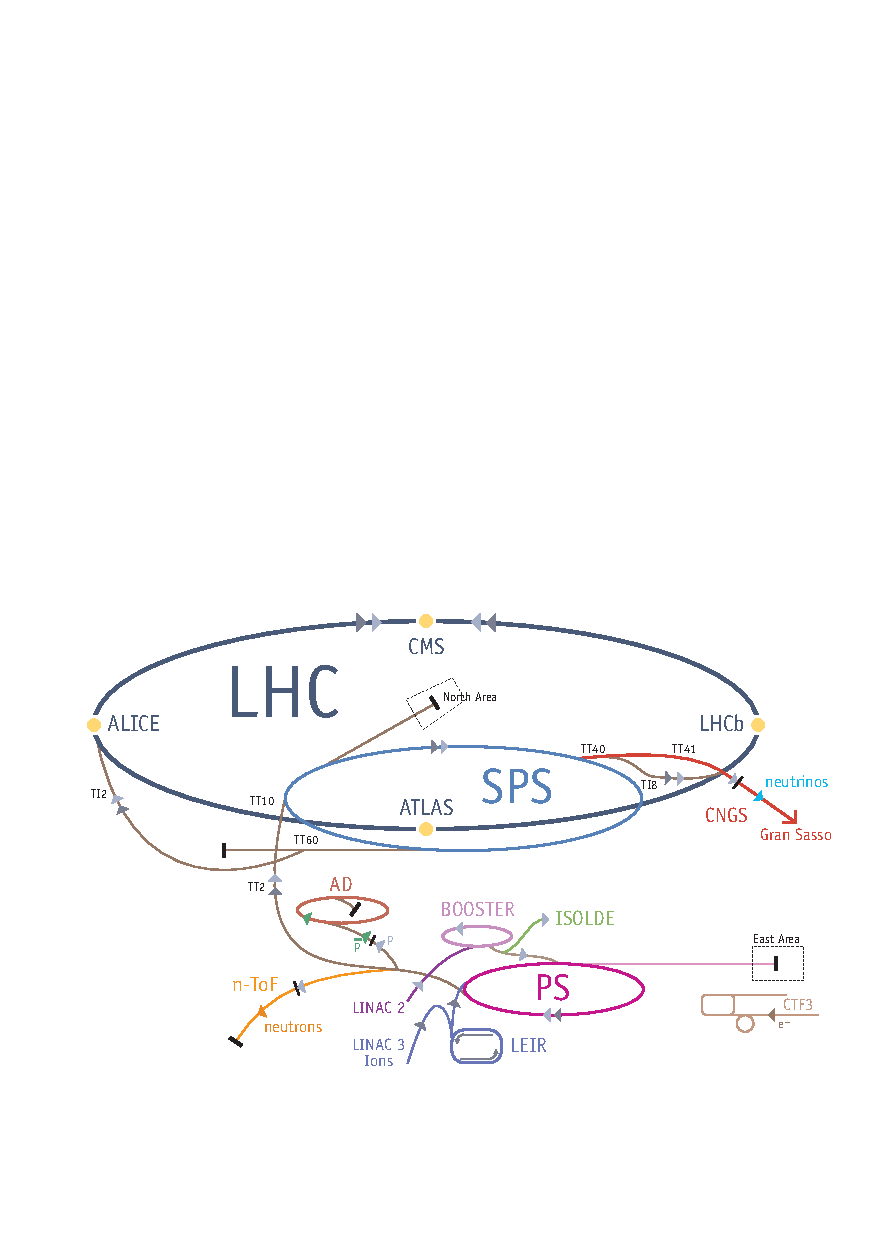
\includegraphics[width=0.90\textwidth]{fig/atlas/accel-chain.pdf}
  \caption{The LHC accelerator complex boosts particles to increasingly higher energies before reaching the LHC. The particle beams are accelerated successively by Linac 2, the Proton Synchrotron Booster (PSB), the Proton Synchrotron (PS), the Super Proton Synchrotron (SPS) and then finally enter the LHC rings~\cite{cern-faq}.}
  \label{fig:lhc-chain}
\end{figure}
\section{Beam conditions}
Due to the Radio Frequency (RF) fields in the accelerating cavities, the proton beams are segmented into groups of protons called \textit{bunches}. Each beam contains 2808 bunches, and each bunch contains 1.7$\times$10$^{11}$ protons. Many protons are included per bunch to maximize the probability of a proton-proton collision for a given bunch crossing. A bunch crossing occurred every 50 nanoseconds during operations in 2012.

Given two equally bunched beams, the instantaneous \textit{luminosity} ($\mathcal{L}$) is given by:
\begin{equation}\label{eqn:lumi}
  \mathcal{L} = f \frac{n_1 n_2}{4\pi \sigma_x\sigma_y},
\end{equation}
where $f=\SI{11245.5}{\hertz}$ is the collision frequency of the LHC beams; $n_{1}$ and $n_{2}$ are the numbers of protons in each beam; and $\sigma_{x}$ and $\sigma_{y}$ are the RMS beam widths in the horizontall (bend) and vertical directions.\cite{PDG} The maximum instantaneous luminosity of the LHC in 2012 was 7.7$\times$10$^{33}$

The instaneous luminosity must be integrated over time because the beam conditions that go into Equation~\ref{eqn:lumi} are always changing over the duration of a run. The integral over time and varied beam conditions is called the integrated luminosity and can be used to relate the number of events $N$ for a given physics process to its cross section $\sigma$:
\begin{equation}\label{eqn:nevt}
  N = \sigma \times \int{\mathcal{L}(t) dt}
\end{equation}
In 2012, the total integrated luminosity of the LHC was 20.3$^{-1}$fb with uncertainty of 2.8\% \cite{Lumi}. The cumulative luminosity recorded over the course of 2012 is shown in Figure~\ref{fig:2012lumi}.
\begin{figure}[tp]
  \centering
  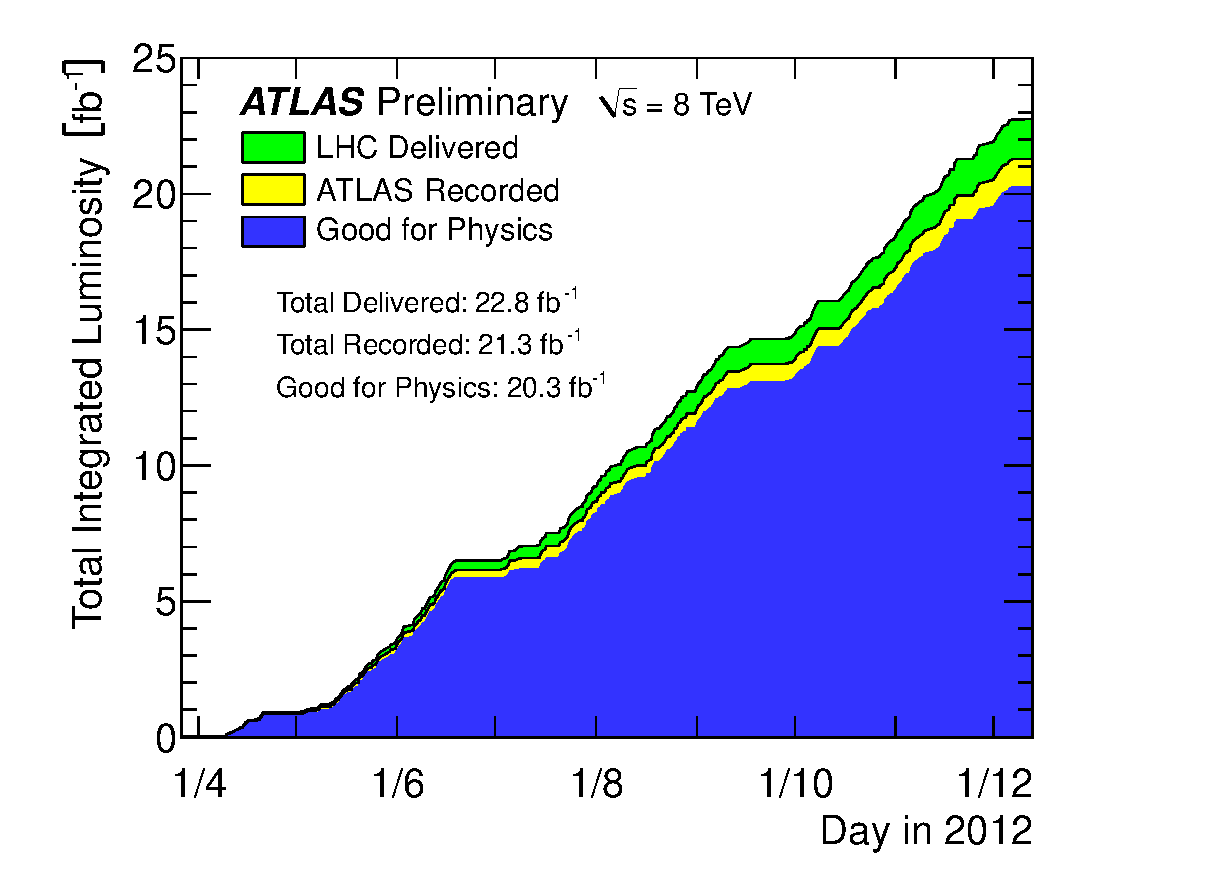
\includegraphics[width=0.90\textwidth]{fig/atlas/intlumivstime2012DQ.eps}
  \caption{Cumulative luminosity versus time delivered to (green), recorded by ATLAS (yellow), and certified to be good quality data (blue) during stable beams and for pp collisions at 8 TeV centre-of-mass energy in 2012. Luminosity can be lost due to data acquisition inefficiency or other effects.}
  \label{fig:2012lumi}
\end{figure}

The beam conditions also determine the number of proton-proton interactions that occur in each bunch crossing. When a single bunch crossing produces multiple separate proton-proton collisions, these events are referred to as \textit{pile-up}. Pile-up presents a signifigant challenge since it can rapidly increase the combinatoric complexity of reconstructing events and quickly degrades the performance of the reconstruction algorithms. In 2012, pile-up was much larger than anticipated. Figure~\ref{fig:pileup} shows the mean number of interactions per bunch crossing for 2011 and 2012, demonstrating the substantial increase of pile-up events in the latter. Reconstruction challenges were overcome by optimizing the existing reconstruction algorithms, as well as new techniques for subtracting pile-up events from the physics of interest. Pile-up techniques used in this analysis will be discussed in the chapter on extra jet object selection.

\begin{figure}[tp]
  \centering
  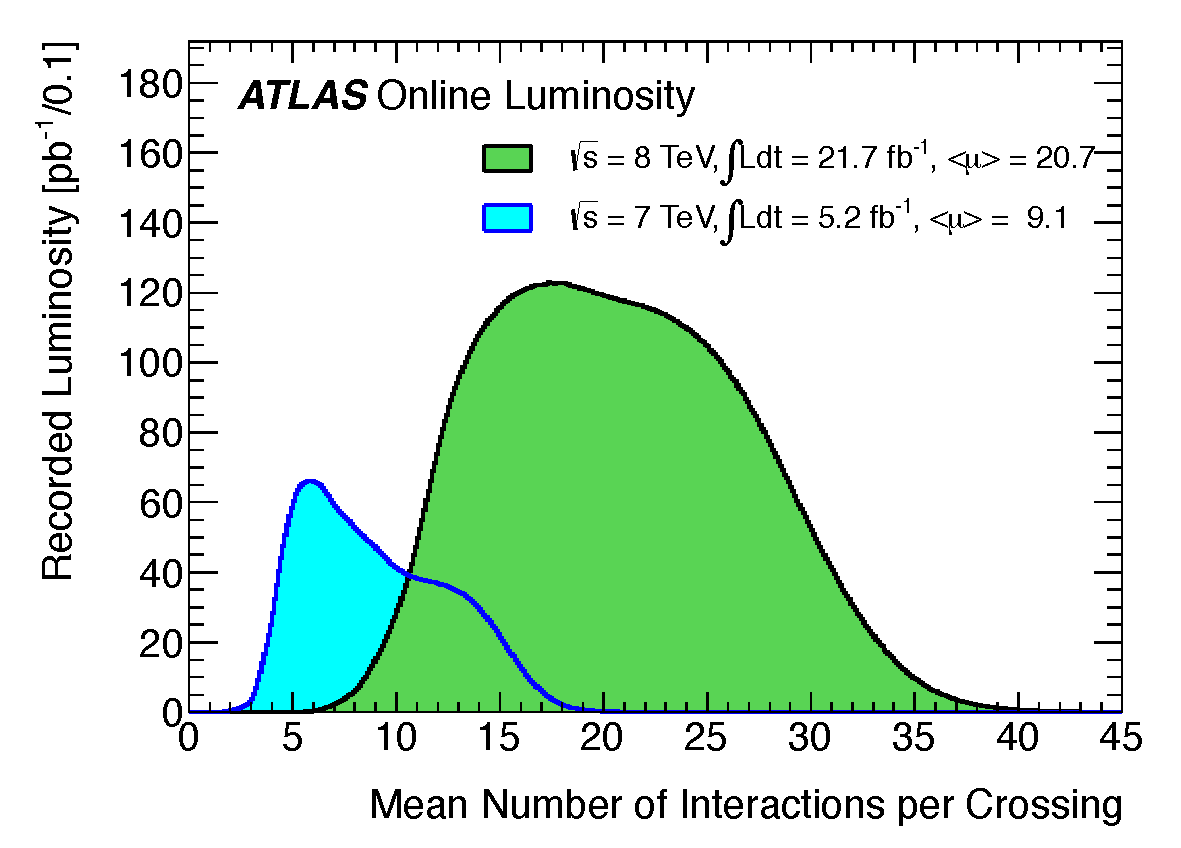
\includegraphics[width=0.90\textwidth]{fig/atlas/pileup.pdf}
  \caption{Luminosity-weight distribution of the mean number of interactions per bunch crossing. Both the full data from the 2011 and 2012 $pp$ runs at the LHC are shown.}
  \label{fig:pileup}
\end{figure}



\section{Overview of the ATLAS detector}
\section{Inner detector}
\subsection{Pixel detector}
\subsection{SemiConductor Tracker}
\subsection{Transition Radiation Tracker}
\subsection{Track reconstruction}
\section{Calorimeters}
\subsection{Electromagnetic calorimeter}
\subsection{Hadronic calorimeter}
\section{Muon spectrometer}
\section{The trigger system}
\subsection{Electron trigger}
\subsection{Muon trigger}